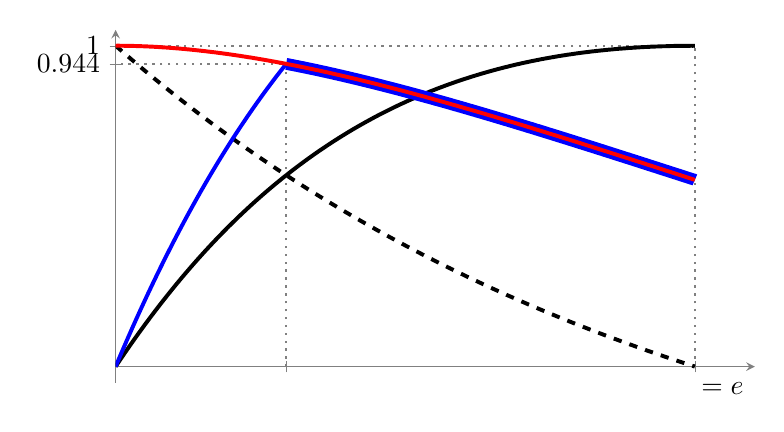
\begin{tikzpicture}[scale=1, transform shape]
\begin{axis}[
axis line style=gray,
axis lines=middle,
xlabel = {$\val$},
xtick={0, 0.800662, 2.7182818284},
ytick={0, 0.943472496484, 1},
xticklabels={0, $\fprice$, ~~~~~~$\optreserve = e$},
yticklabels={0, 0.944, $1$},
xmin=0,xmax=3.0,ymin=-0.05,ymax=1.05,
width=0.8\textwidth,
height=0.5\textwidth,
samples=500]


\addplot[dotted, gray, line width=0.3mm] (2.7182818284, 0) -- (2.7182818284, 1) -- (0, 1);
\addplot[dotted, gray, line width=0.3mm] (0.800662, 0) -- (0.800662, 0.943472496484) -- (0, 0.943472496484);

\addplot[domain=0:2.7182818284, black!100!white, line width=0.5mm] (x, {x*(exp(-x/exp(1)))});

\addplot[domain=0:2.7182818284, dashed, black!100!white, line width=0.5mm] (x, {(1+(exp(-x/exp(1))*(x+exp(1)) - 2)-x*(exp(-x/exp(1))))/1.71828182846});


\addplot[domain=0.800662:2.7182818284, blue, line width=1.5mm] (x, {(1+(exp(-x/exp(1))*(x+exp(1)) - 2)-0*x*(exp(-x/exp(1))))/1.71828182846});
\addplot[domain=0:0.800662, blue, line width=0.5mm] (x, {((1+1.71828182846)*x*(exp(-x/exp(1))))/1.71828182846});


\addplot[domain=0:2.7182818284, red, line width=0.5mm] (x, {(1+(exp(-x/exp(1))*(x+exp(1)) - 2)-0*x*(exp(-x/exp(1))))/1.71828182846});

\end{axis}

\end{tikzpicture}